\subsubsection{Respuesta la escalón para pequeña señal}

\Flor{El escalón de salida quedó con un offset, esto pasó por cambiar el cap de 1m por el de 10u, pero era necesario para determinar la fl.}

\HgraficarPNG{0.5}{sim_rta_escalon_peque.png}{Respuesta al escalón en pequeña señal.}{fig:rta_escalon_peque}

%\begin{figure}[H]
%	\centering
%	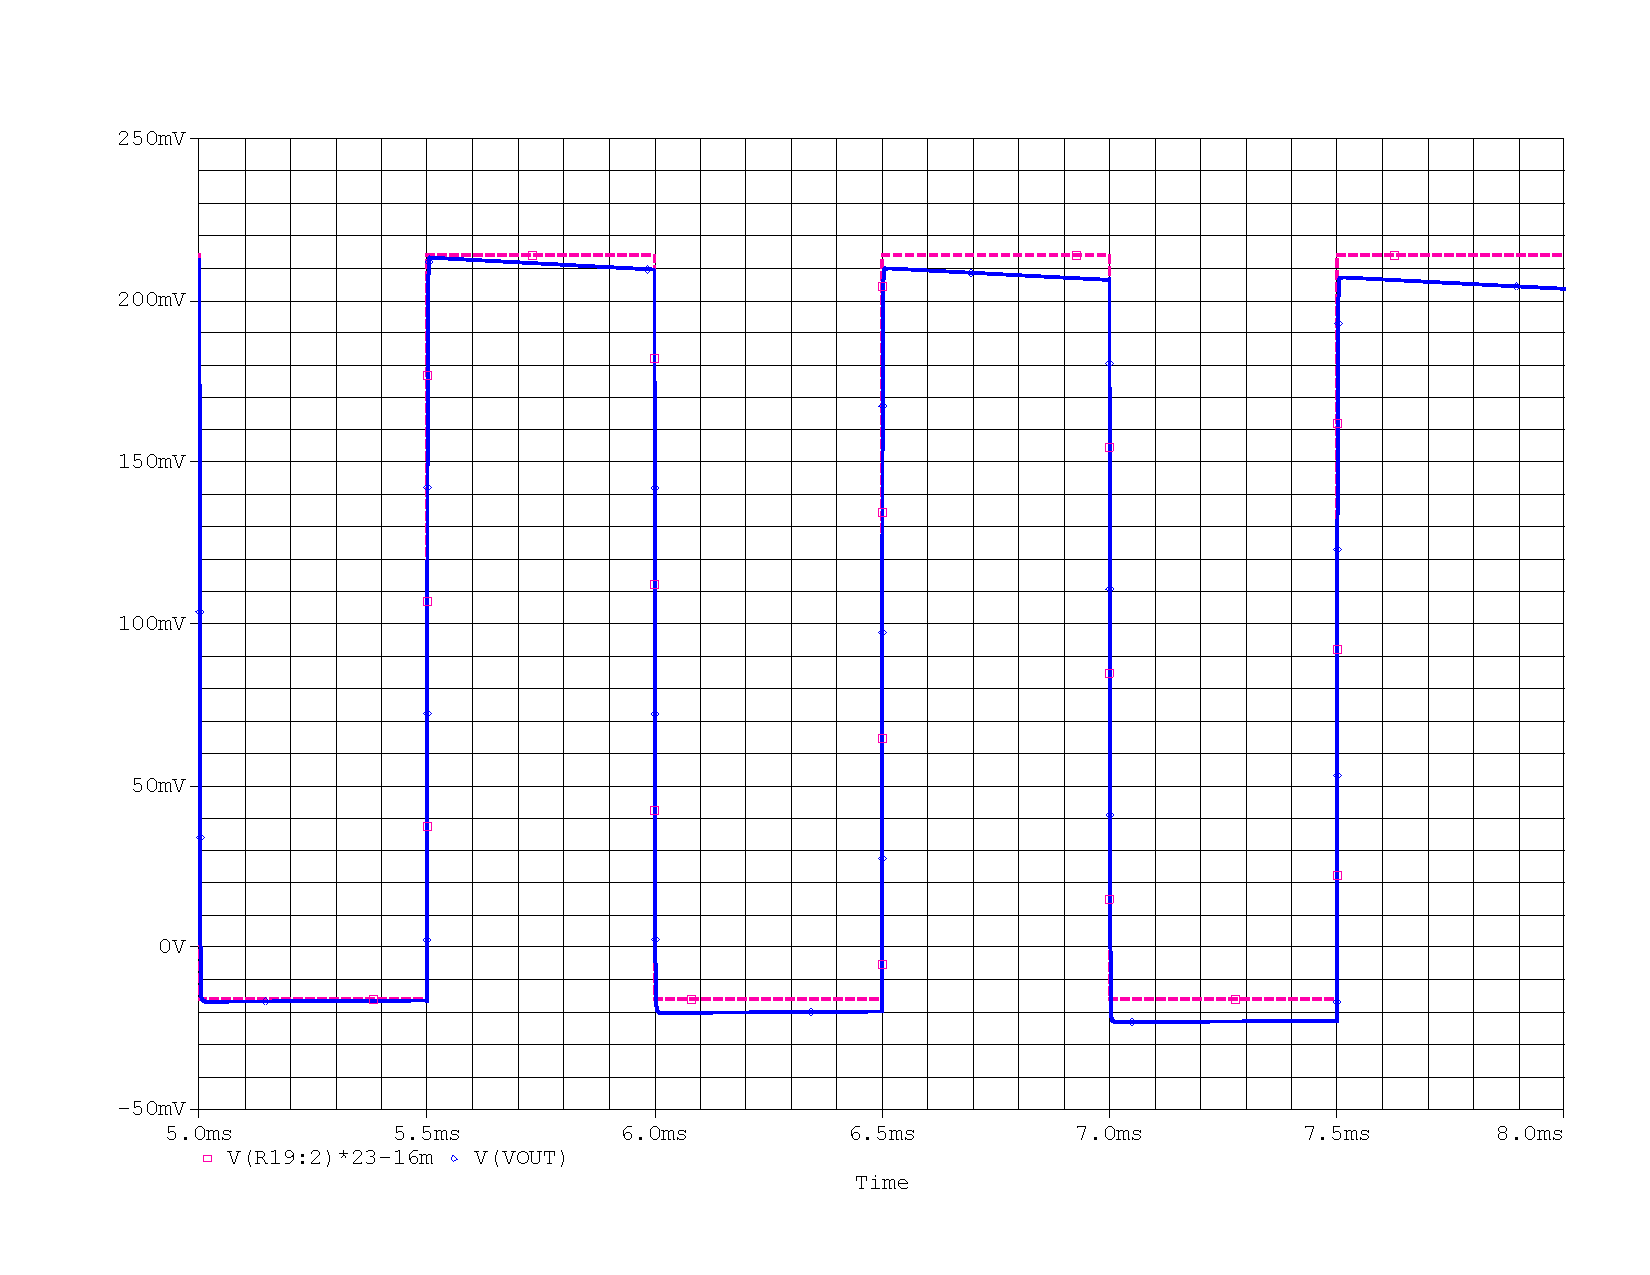
\includegraphics[scale=0.4]{sim_rta_escalon_senial_peque.pdf}
%	\caption{Respuesta al escalón en pequeña señal.}
%	\label{fig:rta_escalon_peque}
%\end{figure}

\subsubsection{Respuesta al escalón para gran señal}

\HgraficarPNG{0.5}{sim_rta_escalon_gran.png}{Respuesta al escalón en gran señal.}{fig:rta_escalon_gran}

%\begin{figure}[H]
%	\centering
%	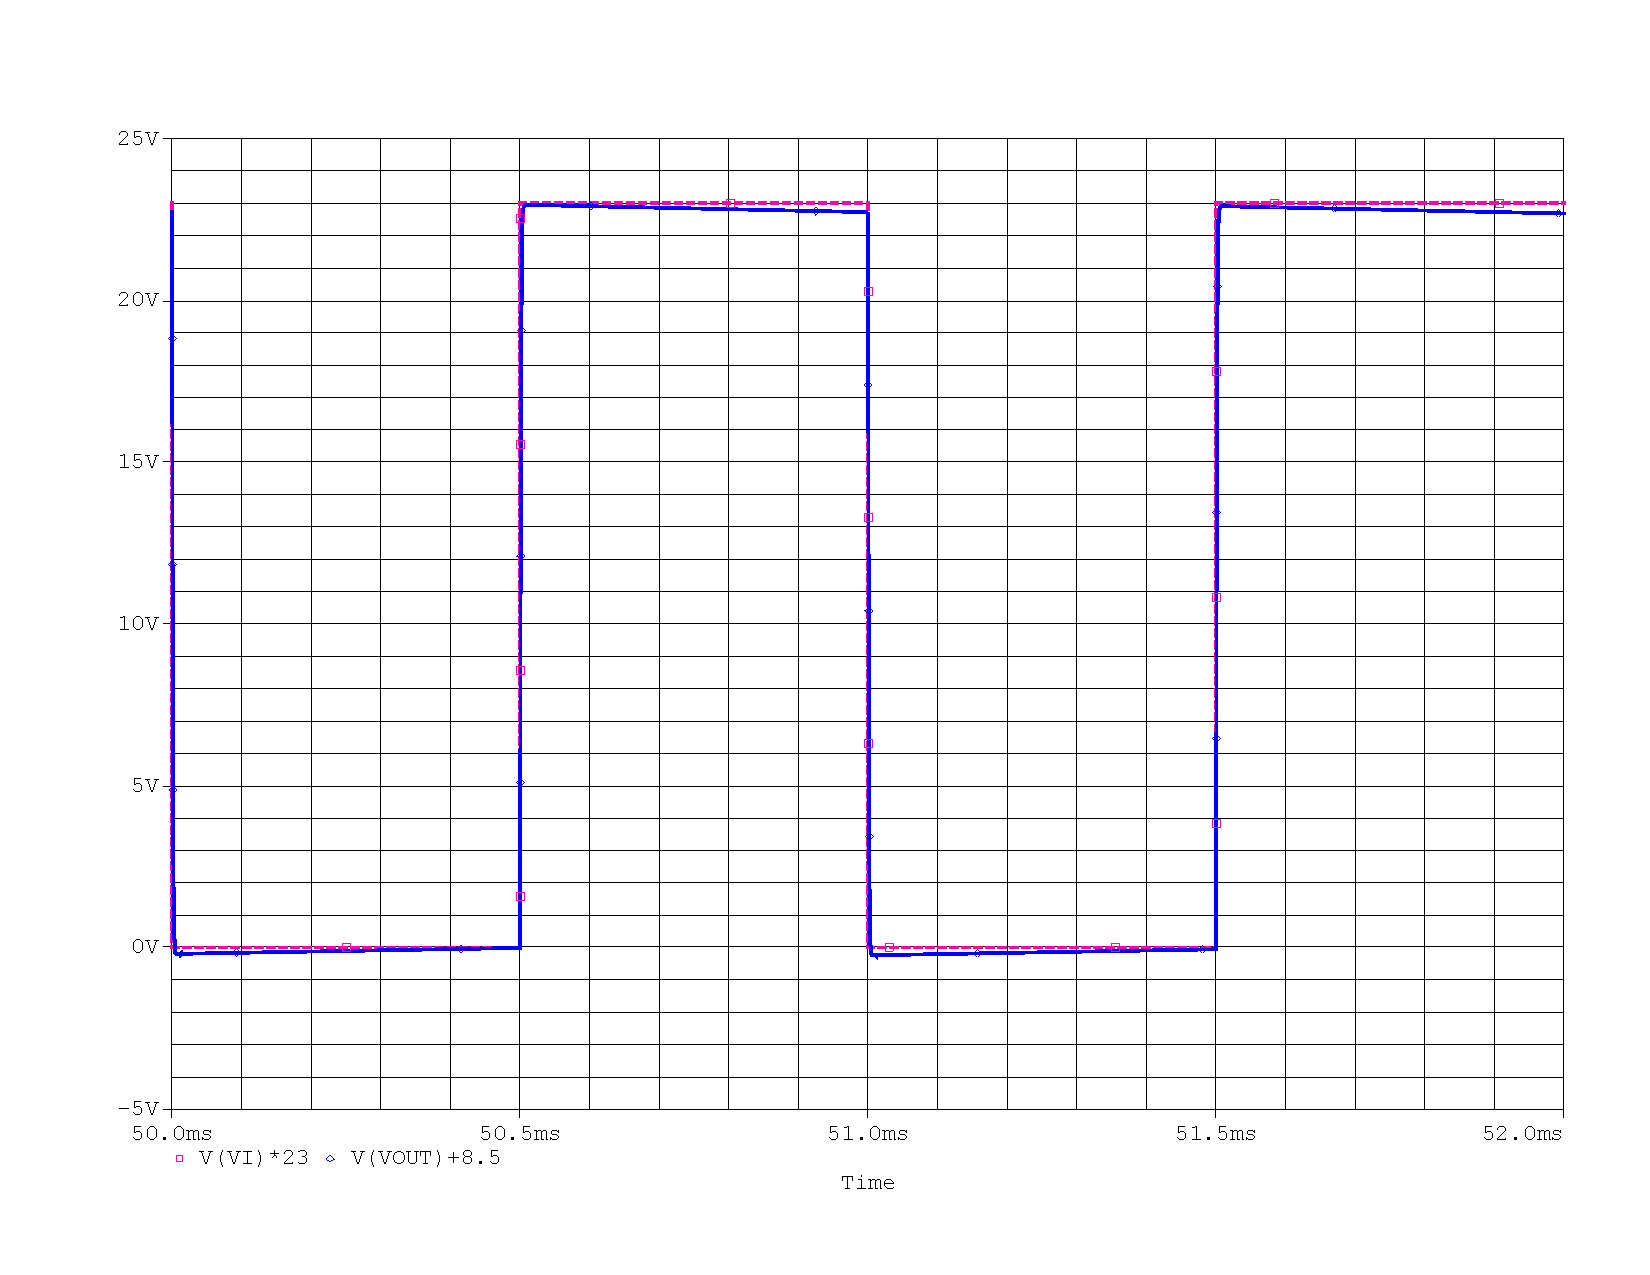
\includegraphics[scale=0.4]{sim_rta_escalon_gran_senial.pdf}
	%\caption{Respuesta al escalón en gran señal.}
	%\label{fig:rta_escalon_gran}
%\end{figure}

\subsubsection{Ancho de banda}

	Este parámetro se obtiene a partir de la simulación de la respuesta al escalón del circuito en pequeña señal (\SI{10}{\milli\volt}).
	
	\HgraficarPNG{0.5}{sim_rta_escalon_gran_zoom.png}{Respuesta al escalón en pequeña señal.}{fig:rta_escalon_peque}

%\begin{figure}[H]
%	\centering
%	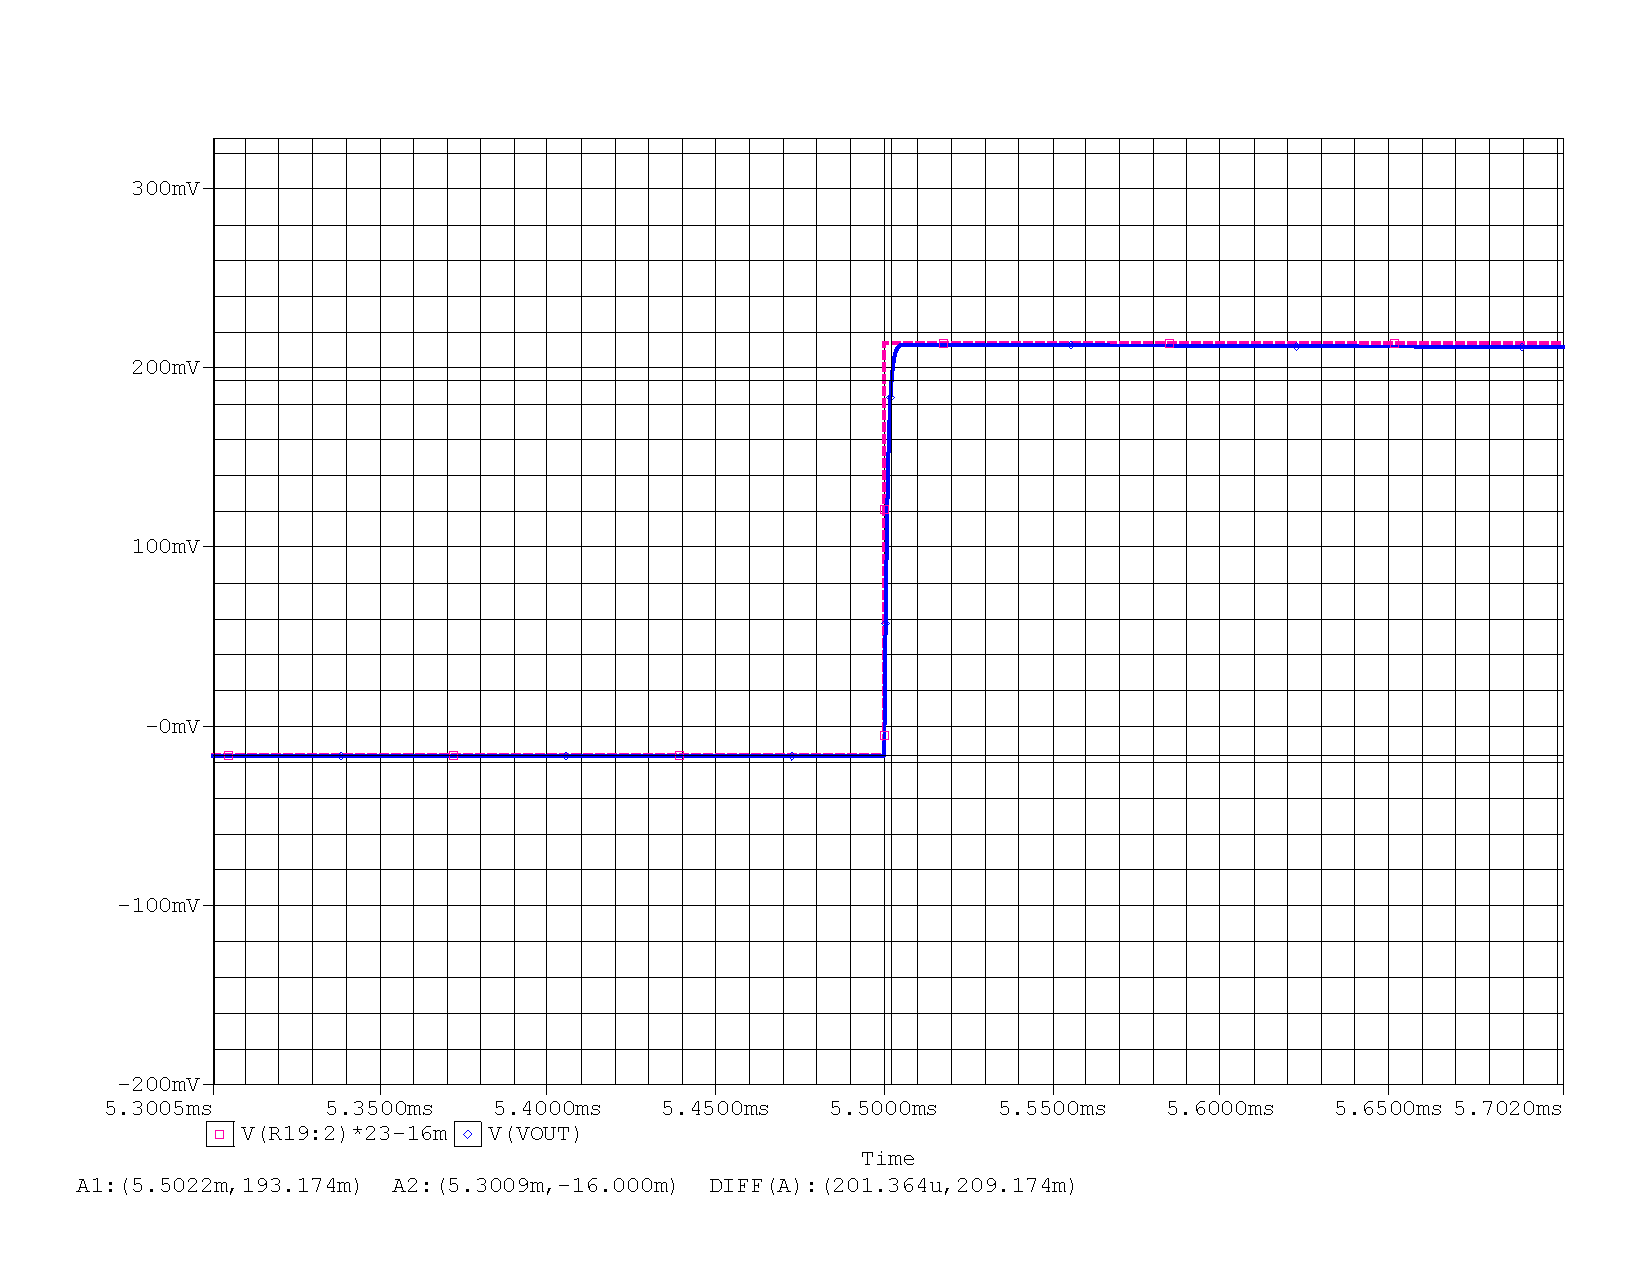
\includegraphics[scale=0.4]{sim_rta_escalon_senial_peque_zoom.pdf}
% 	\caption{Respuesta al escalón en pequeña señal.}
%	\label{fig:rta_escalon_peque}
%\end{figure}

	Observando la figura \ref{fig:sim_bw} el tiempo de crecimiento ($\tau_r$), se puede determinar el ancho de banda mediante la ecuación \eqref{ec:bw}.

	\begin{equation}
		\centering
		\mathrm{BW} = \frac{\num{0,35}}{\tau_r} = \frac{0,35}{\SI{2}{\micro\second}} = \boxed{\SI{175}{\kilo\hertz}}
		\label{ec:bw}
	\end{equation}

\subsubsection{\textit{Slew Rate}}

\HgraficarPNG{0.5}{sim_rta_escalon_gran_zoom.png}{Respuesta al escalón en gran señal ampliado.}{fig:sim_rta_escalon_gran_sr}

%\begin{figure}[H]
%	\centering
%	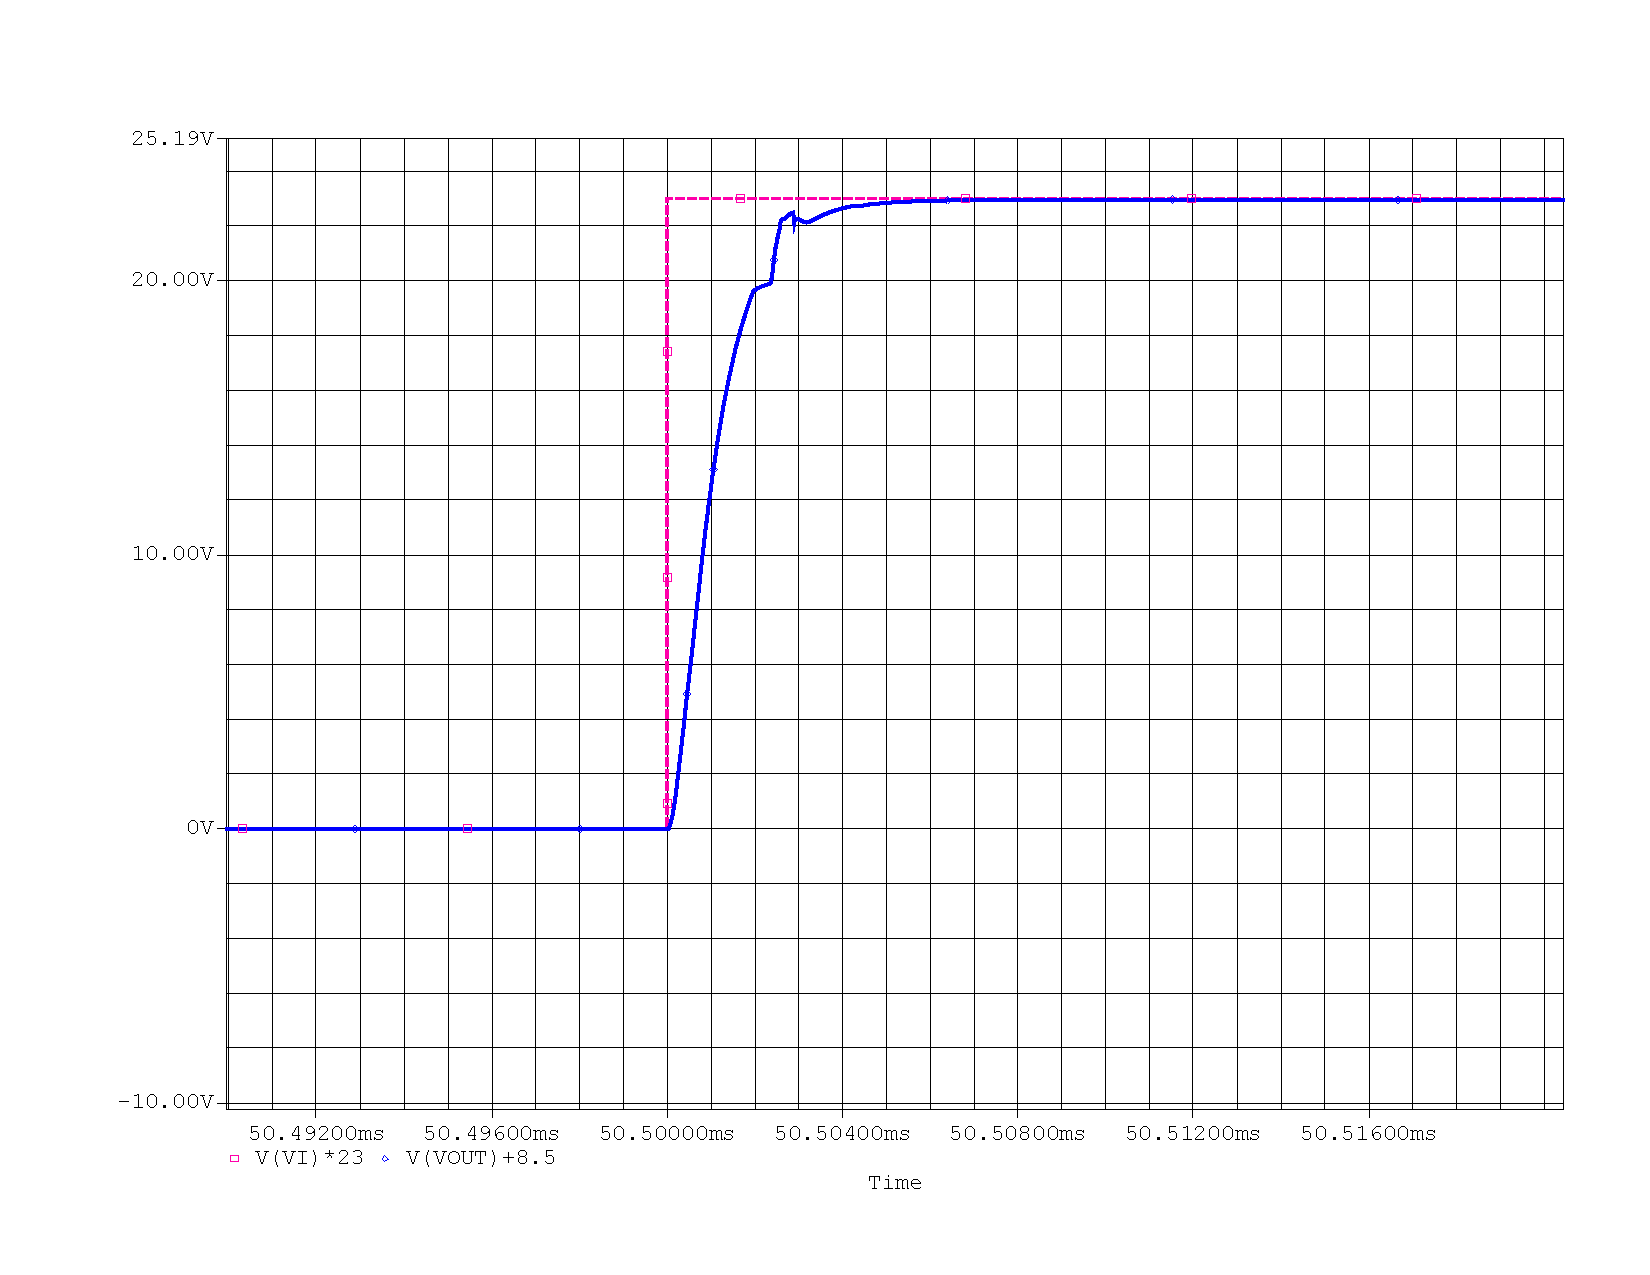
\includegraphics[scale=0.4]{sim_rta_escalon_gran_senial_zoom_sr.pdf}
%	\caption{Respuesta al escalón en gran señal ampliado.}
%	\label{fig:sim_rta_escalon_gran_sr}
%\end{figure}

	El parámetro \textit{Slew Rate} caracteriza el comportamiento de la salida del cirucito ante cambios súbitos de tensión en la entrada, ya que la tensión de salida no puede responder de forma instantánea ante alteraciones en la entrada. Para hallar su valor se impone un escalón en la entrada de gran amplitud y se mide la pendiente casi constante resultante. A partir de la figura \ref{fig:sim_rta_escalon_gran_sr} se obtiene \eqref{ec:sr}.

	\begin{equation}
	\centering
	\mathrm{SR} = \left. \frac{dV_o(t)}{dt} \right\rvert_{max} \cong \frac{\Delta V_o}{\Delta t} = \frac{\SI{27}{\volt}}{\SI{3}{\micro\second}} = \boxed{\SI{9}{\volt\per\micro\second}}
	\label{ec:sr}
\end{equation}


